% paper/sections/12u11_constrained_face_state_space.tex
%
% U11: constrained face-state space gate — Tier IX
% ═══════════════════════════════════════════════════════════════════════════════
\subsubsection{U11：制約 face-state 空間 [Tier IX]}
\label{sec:U11_constrained_face_state_space}

\paragraph{検証対象．}
壁付き計算では，速度の主状態は任意の face cochain ではなく
\[
  F_w=\ker C_w,\qquad C_w=B_wR_h
\]
に属する必要がある（式~\eqref{eq:wall_constrained_face_space}）．
U11 は，metric retraction $P_w$（式~\eqref{eq:wall_metric_retraction}）と
制限圧力勾配 $G_w=P_wG_A$（式~\eqref{eq:restricted_pressure_operator}）が，
小型製造 probe 上で状態空間 gate を満たすことを確認する．
periodic-wall では full array endpoint を独立自由度として扱わず，
式~\eqref{eq:periodic_wall_quotient_complex} と
式~\eqref{eq:periodic_wall_quotient_rank_gate} の quotient 空間で rank を読む．

\paragraph{設定．}
full-wall と $x$ 周期・$y$ 壁の小型格子で，
乱数 face state と乱数圧力を用いて以下を測る：
\[
  C_wP_w f=0,\qquad P_w^2=P_w,\qquad
  \langle P_wa,b\rangle_M=\langle a,P_wb\rangle_M,
\]
\[
  \langle P_wG_Ap,\eta\rangle_M+\langle p,D_f\eta\rangle_W=0
  \quad(\eta\in F_w),
\]
および
\[
  \operatorname{rank}(D_wP_wG_A)=\operatorname{rank}(D_w|_{F_w}) .
\]
負対照として，境界面だけを zero clamp する post-clamp と，
periodic endpoint を独立圧力自由度として持つ full-array mode を拒否する．

\paragraph{結果．}

\begin{table}[!ht]
\caption{U11：制約 face-state 空間 gate}
\label{tab:U11_constrained_face_state_space}
\PaperCaptionNote{wall は full-wall topology，periodic-wall は quotient pressure/face topology で評価する．rank 列は $\operatorname{rank}(D_w|_{F_w})/\operatorname{rank}(D_wP_wG_A)$．}
\centering\small
\begin{tabular}{l c c c c c}
\toprule
BC & $\|C_wP_wf\|_\infty$ & $\|P_w^2f-P_wf\|_2$ & 自己随伴 rel. & Green rel. & rank \\
\midrule
wall & $2.581\times10^{-12}$ & $4.851\times10^{-12}$ & $8.707\times10^{-14}$ & $1.294\times10^{-16}$ & $19/19$ \\
periodic-wall & $1.277\times10^{-15}$ & $0.000\times10^{0}$ & $6.009\times10^{-17}$ & $1.095\times10^{-16}$ & $25/25$ \\
\bottomrule
\end{tabular}
\end{table}

\begin{figure}[!ht]
\centering
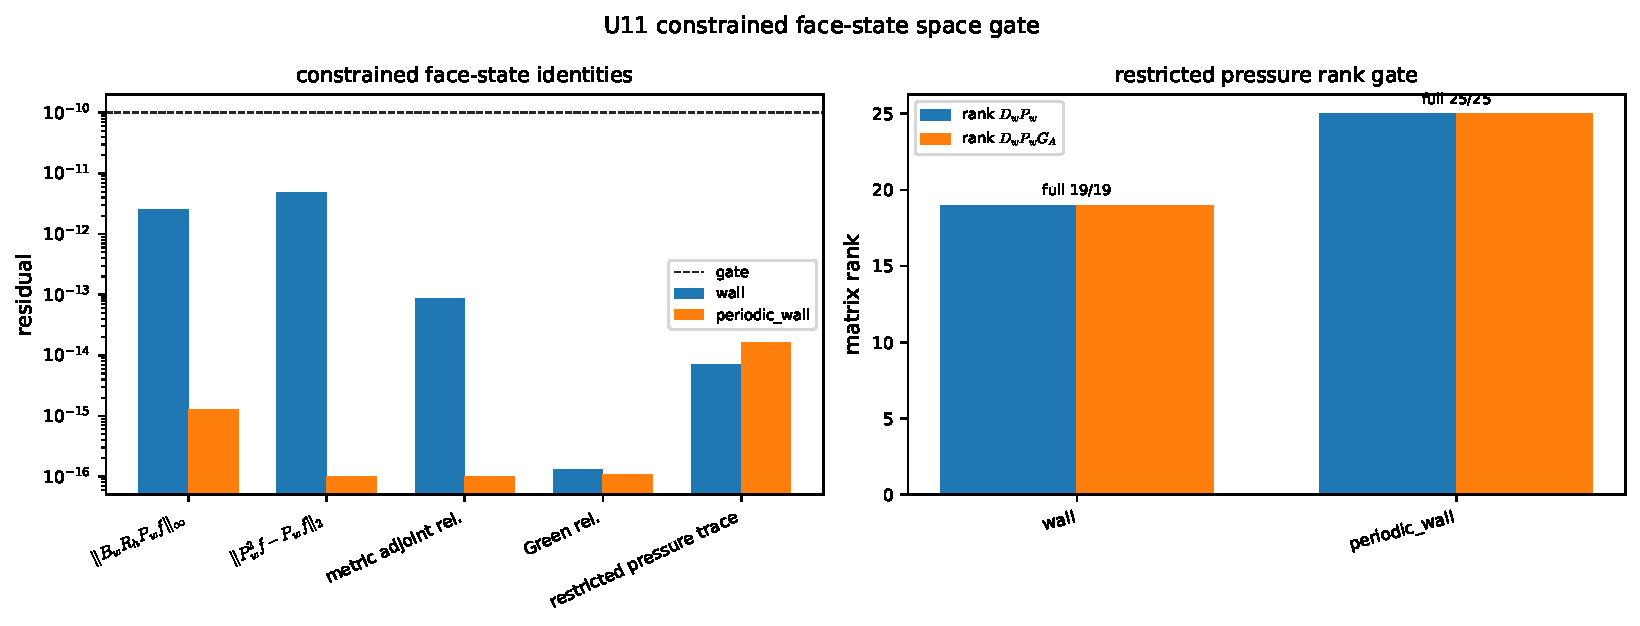
\includegraphics[width=0.96\linewidth]{figures/ch12_u11_constrained_face_state_space}
\caption{U11：制約 face-state 空間 gate}
\label{fig:ch12_u11_constrained_face_state_space}
\PaperCaptionNote{左：$P_w$ の wall trace，冪等性，metric self-adjointness，制限 Green identity は丸め誤差まで閉じる．右：restricted divergence と restricted pressure operator の rank が wall と periodic-wall quotient の双方で一致する．full endpoint 表示は表示上の負対照であり，periodic pressure は quotient 空間で読む．}
\end{figure}

\paragraph{負対照．}
境界面だけを zero clamp した post-clamp は wall trace を消せず，
最大 trace は wall で $1.375$，periodic-wall で $0.986$ であった．
また periodic endpoint を独立にずらす full-array pressure mode は
endpoint gap $2.0$ と制限 flux norm $22.14$ を持ち，quotient 圧力変数としては受理しない．
したがって U11 は，post-pressure 壁修復や nodal/endpoint clamp を
$P_w$ の代替として採用しない負の知識も同時に固定する．

\paragraph{判定と次章への接続．}
U11 は \checkmark と判定する．
これは $F_w$ と periodic-wall quotient の component gate であり，
第13章に新しい V11 physical benchmark を追加する根拠ではない．
V6/V7/V9 は引き続き壁付き pressure-jump/HFE 結合系の統合検証として読み，
periodic-wall の有限振幅 rising-bubble 応答は第~\ref{sec:benchmarks}章へ送る．

\FloatBarrier
